\chapter{线性代数}
\label{chap:linear-algebra}

第~\ref{part:mathematical-language-analysis-optimization}部分已经多次使用向量和矩阵：参数写成向量，导数给出局部线性近似，最小二乘把一组预测与观测作比较。但同一串数字有时表示空间中的对象，有时只是对象在某组基下的坐标；同一个线性映射换一组坐标后会得到不同的矩阵；两个特征几乎重复时，预测结果可能变化不大，表示它的系数却会剧烈变化。若不区分这些层次，公式虽然能够相乘，所得结论却未必对应原来的问题。

本章用一组近共线特征贯穿这些区别。令
\begin{equation}
  \bm{X}_{\varepsilon} = \begin{bmatrix} 1 & 1 \\ 1 & 1+\varepsilon \\ 1 & 1-\varepsilon \end{bmatrix} = \begin{bmatrix} \bm{c}_1 & \bm{c}_2 \end{bmatrix}, \qquad \bm{q} = \begin{bmatrix} 0\\1\\-1 \end{bmatrix}, \label{eq:linear-algebra-nearly-collinear-design}
\end{equation}
其中$\bm{c}_1=(1,1,1)^{\top}$且$\bm{c}_2=\bm{c}_1+\varepsilon\bm{q}$。当$\varepsilon\neq0$时，两列线性无关；当$\varepsilon=0$时，它们完全重合。只要$|\varepsilon|$很小，两列的夹角便很小，因而称为\term{近共线}（nearly collinear）。这不是说样本点彼此接近，而是说作为$\mathbb{R}^3$中向量的两列特征接近同一个方向。

要判断近共线究竟影响对象还是坐标，需要把抽象向量、基和矩阵表示分开；要比较拟合误差，
还必须选定范数与内积。投影与最小二乘把这些结构接到观测拟合，多维数组与缩并再将同样的
线性运算扩展到多个索引。不同方向被映射放大多少、近共线为何造成数值敏感，以及秩不足时
怎样选择最小范数系数，则需要下一章的谱与奇异值工具。

\section{向量空间与坐标}
\label{sec:linear-algebra-vector-spaces-coordinates}

\subsection{向量空间与线性运算}

向量不必天然是一列数字。位移、有序信号、函数和矩阵都可以相加，也可以乘一个标量；只要这些运算满足共同规则，就能作为同一种代数对象处理。设$\mathbb{F}$表示标量域，本书主要使用实数域$\mathbb{R}$，涉及频率表示时也会使用复数域$\mathbb{C}$。\term{向量空间}（vector space）$V$是一个集合，其上定义了向量加法与标量乘法，并且对任意$\bm{u},\bm{v},\bm{w}\in V$和$a,b\in\mathbb{F}$满足
\[
  \bm{u}+\bm{v}\in V,\qquad
  a\bm{u}\in V,
\]
以及加法的结合律和交换律、零向量与加法逆元的存在、标量乘法的结合律和分配律，并有$1\bm{v}=\bm{v}$。这些条件的作用是保证有限次线性运算不会离开$V$。

例如，$\mathbb{R}^d$在逐坐标加法和数乘下是实向量空间；所有$m\times d$实矩阵组成的集合$\mathbb{R}^{m\times d}$也是实向量空间。次数不超过$k$的实系数多项式同样构成向量空间，因为两个这类多项式相加或数乘后，次数仍不超过$k$。相比之下，
\[
  H=\{\bm{x}\in\mathbb{R}^d:x_1=1\}
\]
不是通常运算下的向量空间：它不包含零向量，而且两个元素相加后的第一坐标为$2$。集合是否“看起来像一条直线或一个平面”并非判断标准，封闭性与向量空间公理才是。

若$U\subseteq V$在$V$的加法和数乘下本身构成向量空间，就称$U$为$V$的\term{线性子空间}（linear subspace）。验证非空集合$U$为子空间时，可以合并检查为
\[
  \forall \bm{u},\bm{v}\in U,\ \forall a,b\in\mathbb{F},
  \qquad a\bm{u}+b\bm{v}\in U.
\]
取$a=b=0$可见零向量必须在$U$中。因而不过原点的仿射直线不是线性子空间，即使它仍能用少量坐标描述。

\subsection{张成与线性无关}

给定$\bm{v}_1,\ldots,\bm{v}_k\in V$，形如
\[
  a_1\bm{v}_1+\cdots+a_k\bm{v}_k,
  \qquad a_1,\ldots,a_k\in\mathbb{F},
\]
的向量称为它们的\term{线性组合}（linear combination）。所有线性组合组成的集合
\[
  \operatorname{span}\{\bm{v}_1,\ldots,\bm{v}_k\}
  =
  \left\{
    \sum_{j=1}^{k}a_j\bm{v}_j:a_j\in\mathbb{F}
  \right\}
\]
是包含这些向量的最小线性子空间，称为它们的\term{张成空间}（span）。“能否表示目标对象”由目标是否属于张成空间决定。

覆盖空间并不意味着表示唯一。若
\begin{equation}
  a_1\bm{v}_1+\cdots+a_k\bm{v}_k=\bm{0} \label{eq:linear-algebra-independence-relation}
\end{equation}
只在$a_1=\cdots=a_k=0$时成立，就称这组向量\term{线性无关}（linearly independent）。否则，其中至少一个非零系数参与了式\eqref{eq:linear-algebra-independence-relation}；选取一个非零的$a_j$并移项，便能把$\bm{v}_j$写成其余向量的线性组合。线性相关因此准确表达了表示中的冗余，而不只是两个向量恰好相等。

式~\eqref{eq:linear-algebra-nearly-collinear-design}给出了一个可以直接核对的例子。若
\[
  a_1\bm{c}_1+a_2\bm{c}_2
  =
  (a_1+a_2)\bm{c}_1+a_2\varepsilon\bm{q}
  =
  \bm{0},
\]
由于$\bm{c}_1$的三个坐标相同，而$\bm{q}$的后两个坐标符号相反，$\bm{c}_1$与$\bm{q}$线性无关。当$\varepsilon\neq0$时，只能有$a_2=0$和$a_1=0$，所以$\bm{c}_1,\bm{c}_2$线性无关。当$\varepsilon=0$时，$\bm{c}_2=\bm{c}_1$，取$(a_1,a_2)=(1,-1)$便得到非平凡关系。近共线与线性相关不是一回事：前者描述接近退化的程度，后者是一个精确的是非判断。

\subsection{基与坐标}

向量空间$V$的一组向量若既线性无关又张成$V$，就称为$V$的一组\term{基}（basis）。设$\mathcal{B}=(\bm{b}_1,\ldots,\bm{b}_d)$是一组有序基。每个$\bm{v}\in V$都能唯一写成
\[
  \bm{v}
  =
  x_1\bm{b}_1+\cdots+x_d\bm{b}_d.
\]
系数组成的列向量
\[
  [\bm{v}]_{\mathcal{B}}
  =
  (x_1,\ldots,x_d)^{\top}\in\mathbb{F}^d
\]
称为$\bm{v}$在基$\mathcal{B}$下的\term{坐标}（coordinates）。存在性来自基的张成性质；若有两组坐标，相减后得到式\eqref{eq:linear-algebra-independence-relation}形式的关系，线性无关性又保证两组系数相同。

一组基所含向量的个数称为有限维空间的\term{维数}（dimension），记作$\dim V$。同一有限维空间的任意两组基所含向量数相同，因此维数不依赖具体坐标选择。$\mathbb{R}^d$的标准基是$\bm{e}_1,\ldots,\bm{e}_d$，其中$\bm{e}_j$只有第$j$个坐标为$1$。平常把向量直接写成数字列，实际是在默认使用这组标准基。

若$V$能由有限个向量张成，就可以从一组有限生成向量中反复删除可由其余向量表示的成员，直至得到一组基。因此每个有限维向量空间都有基。更一般地，$V$中的任意线性无关组都能通过加入向量扩充为一组基；这也说明后文从子空间的基扩充到整个空间的基是合法的。第~\ref{chap:functional-analysis-and-approximation}章式~\eqref{eq:functional-finite-basis-expansion}中的基函数展开正是同一坐标关系：函数是向量空间中的对象，系数列是它在所选函数基下的坐标。

对象与坐标的区别在近共线例子中尤其重要。固定$\delta=0.1$并令
\begin{equation}
  \bm{y} = \bm{c}_1+\delta\bm{q} = \begin{bmatrix} 1\\1.1\\0.9 \end{bmatrix}. \label{eq:linear-algebra-nearly-collinear-target}
\end{equation}
在基$\mathcal{B}_0=(\bm{c}_1,\bm{q})$下，$[\bm{y}]_{\mathcal{B}_0}=(1,\delta)^{\top}$。若$\varepsilon\neq0$，同一个子空间也可用$\mathcal{B}_{\varepsilon}=(\bm{c}_1,\bm{c}_2)$作为基。由$\bm{q}=(\bm{c}_2-\bm{c}_1)/\varepsilon$可得
\begin{equation}
  \bm{y} = \left(1-\frac{\delta}{\varepsilon}\right)\bm{c}_1 + \frac{\delta}{\varepsilon}\bm{c}_2. \label{eq:linear-algebra-coordinate-instability}
\end{equation}
当$\varepsilon=0.01$时，坐标从$(1,0.1)^{\top}$变成$(-9,10)^{\top}$，但空间中的对象$\bm{y}$没有改变。大系数在这里首先反映所选基接近线性相关，不能单凭坐标绝对值断言对象本身很大。

\subsection{换基与坐标变换}

设$\mathcal{B}=(\bm{b}_1,\ldots,\bm{b}_d)$与$\mathcal{C}=(\bm{c}_1,\ldots,\bm{c}_d)$都是$V$的基。把每个$\bm{b}_j$在$\mathcal{C}$下的坐标作为第$j$列，得到换基矩阵
\[
  \bm{S}_{\mathcal{C}\leftarrow\mathcal{B}}
  =
  \begin{bmatrix} [\bm{b}_1]_{\mathcal{C}} & \cdots & [\bm{b}_d]_{\mathcal{C}} \end{bmatrix}.
\]
由于坐标映射保持线性组合，
\begin{equation}
  [\bm{v}]_{\mathcal{C}} = \bm{S}_{\mathcal{C}\leftarrow\mathcal{B}} [\bm{v}]_{\mathcal{B}}. \label{eq:linear-algebra-coordinate-change}
\end{equation}
两组基都能唯一表示对象，所以换基矩阵可逆，其逆是$\bm{S}_{\mathcal{B}\leftarrow\mathcal{C}}$。

在$\mathcal{B}_0=(\bm{c}_1,\bm{q})$与$\mathcal{B}_{\varepsilon}=(\bm{c}_1,\bm{c}_2)$之间，
\[
  \bm{S}_{\mathcal{B}_0\leftarrow\mathcal{B}_{\varepsilon}}
  =
  \begin{bmatrix} 1 & 1\\ 0 & \varepsilon \end{bmatrix}.
\]
它的行列式为$\varepsilon$，在$\varepsilon\neq0$时可逆；随着$\varepsilon$趋近$0$，逆矩阵中的$1/\varepsilon$项增大。这一计算已经揭示坐标敏感性的来源，但要定量比较不同方向上的放大，还需要下一章的奇异值与条件数。

\section{矩阵与线性映射}
\label{sec:linear-algebra-matrices-linear-maps}

坐标给出了一个向量怎样记录，线性映射则说明它怎样变成另一个向量。
本科课程中熟悉的矩阵乘法、逆和行列式，在这里分别对应映射复合、可逆性和体积变化。
随后用像空间与零空间判断方程是否可解；此时尚未选择“最近”的含义，不能直接谈拟合误差。

\subsection{线性映射的矩阵表示}

设$V,W$是同一标量域上的向量空间。映射$T:V\to W$若对任意$\bm{u},\bm{v}\in V$和$a,b\in\mathbb{F}$满足
\[
  T(a\bm{u}+b\bm{v})
  =
  aT(\bm{u})+bT(\bm{v}),
\]
就称为\term{线性映射}（linear map）。它保留线性组合，特别有$T(\bm{0})=\bm{0}$。带有非零偏置的映射$\bm{x}\mapsto\bm{A}\bm{x}+\bm{b}$通常称为仿射映射；只有$\bm{b}=\bm{0}$时才是线性映射。

给定$V$的基$\mathcal{B}=(\bm{b}_1,\ldots,\bm{b}_d)$和$W$的基$\mathcal{C}=(\bm{c}_1,\ldots,\bm{c}_m)$，线性映射完全由各基向量的像决定。把$[T(\bm{b}_j)]_{\mathcal{C}}$作为第$j$列，得到矩阵$[T]_{\mathcal{C}\leftarrow\mathcal{B}}\in\mathbb{F}^{m\times d}$，并有
\begin{equation}
  [T(\bm{v})]_{\mathcal{C}} = [T]_{\mathcal{C}\leftarrow\mathcal{B}} [\bm{v}]_{\mathcal{B}}. \label{eq:linear-algebra-map-matrix-representation}
\end{equation}
矩阵的列数由输入空间维数决定，行数由输出空间维数决定。线性映射是坐标无关的对象，矩阵则依赖输入端和输出端各自选用的基。

设计矩阵$\bm{X}_{\varepsilon}\in\mathbb{R}^{3\times2}$表示线性映射
\[
  T_{\varepsilon}:\mathbb{R}^2\to\mathbb{R}^3,
  \qquad
  T_{\varepsilon}(\bm{w})=\bm{X}_{\varepsilon}\bm{w}.
\]
输入$\bm{w}=(w_1,w_2)^{\top}$给出两列特征的组合系数，输出$w_1\bm{c}_1+w_2\bm{c}_2$是三个样本上的拟合向量。这里输入空间与输出空间不同，所以不能把“系数向量”和“拟合向量”视为同一个对象。

\subsection{矩阵乘法与映射复合}

若$T:U\to V$与$S:V\to W$都是线性映射，则复合$S\circ T:U\to W$仍为线性映射。在相容的基下，其矩阵满足
\[
  [S\circ T]=[S][T].
\]
这解释了矩阵乘法为何按“左矩阵的行乘右矩阵的列”定义。若$\bm{A}\in\mathbb{F}^{m\times d}$且$\bm{B}\in\mathbb{F}^{d\times k}$，那么
\begin{equation}
  (\bm{A}\bm{B})_{i,j} = \sum_{\ell=1}^{d}a_{i,\ell}b_{\ell,j}, \qquad \bm{A}\bm{B}\in\mathbb{F}^{m\times k}. \label{eq:linear-algebra-matrix-product}
\end{equation}
被求和的中间索引$\ell$对应复合映射的中间空间。维度不匹配意味着两个映射不能按该次序复合，而不仅是书写格式有误。

复合的先后通常不能交换。即使$\bm{A}\bm{B}$和$\bm{B}\bm{A}$都能定义，它们也可能不同。例如
\[
  \begin{bmatrix} 1&0\\0&0 \end{bmatrix}
  \begin{bmatrix} 0&1\\1&0 \end{bmatrix}
  =
  \begin{bmatrix} 0&1\\0&0 \end{bmatrix},
  \qquad
  \begin{bmatrix} 0&1\\1&0 \end{bmatrix}
  \begin{bmatrix} 1&0\\0&0 \end{bmatrix}
  =
  \begin{bmatrix} 0&0\\1&0 \end{bmatrix}.
\]
前者先交换坐标再保留第一坐标，后者先保留第一坐标再交换；两个过程的输出自然不同。

\subsection{转置、伴随与逆映射}

实矩阵$\bm{A}\in\mathbb{R}^{m\times d}$的\term{转置}（transpose）$\bm{A}^{\top}\in\mathbb{R}^{d\times m}$交换行列，$(\bm{A}^{\top})_{i,j}=a_{j,i}$。它满足
\[
  (\bm{A}\bm{B})^{\top}=\bm{B}^{\top}\bm{A}^{\top}.
\]
次序反转是因为转置后的映射要按相反方向与内积配对。对复矩阵，还要同时取复共轭，得到\term{共轭转置}（conjugate transpose）$\bm{A}^{*}=\overline{\bm{A}}^{\top}$。实矩阵是复矩阵的特殊情形，此时$\bm{A}^{*}=\bm{A}^{\top}$。

方阵$\bm{A}\in\mathbb{F}^{d\times d}$若存在$\bm{A}^{-1}$使
\[
  \bm{A}^{-1}\bm{A}
  =
  \bm{A}\bm{A}^{-1}
  =
  \bm{I}_d,
\]
就称为可逆矩阵。它表示一个双射线性映射，$\bm{A}^{-1}$表示逆映射。可逆性等价于列向量线性无关，也等价于列向量张成$\mathbb{F}^d$。非方矩阵不能拥有上述双侧逆；某些非方矩阵可以有单侧逆，但这只对应单射或满射中的一项。

同一个线性算子$T:V\to V$在两组基$\mathcal{B}$和$\mathcal{C}$下的矩阵记为$\bm{A}_{\mathcal{B}}$与$\bm{A}_{\mathcal{C}}$。若$\bm{S}=\bm{S}_{\mathcal{C}\leftarrow\mathcal{B}}$，由式\eqref{eq:linear-algebra-coordinate-change}在输入和输出两端各换一次坐标，可得
\begin{equation}
  \bm{A}_{\mathcal{C}} = \bm{S}\bm{A}_{\mathcal{B}}\bm{S}^{-1}. \label{eq:linear-algebra-similarity-change-basis}
\end{equation}
这类矩阵称为相似矩阵。矩阵元素随基改变，但映射是否可逆、像空间维数等性质不变。

\subsection{行列式与体积变化}

对$\bm{A}\in\mathbb{F}^{d\times d}$，\term{行列式}（determinant）$\det(\bm{A})$是一个标量。它可以由三项性质刻画：对每一列分别线性，交换两列会变号，且$\det(\bm{I}_d)=1$。在实坐标中，$\det(\bm{A})$给出有向体积的缩放因子：其绝对值$|\det(\bm{A})|$是普通体积的缩放倍数，其符号则记录定向保持还是反转。

若矩阵列向量线性相关，它们张成的平行多面体被压到更低维空间，体积为零，因而$\det(\bm{A})=0$。反过来，$\det(\bm{A})\neq0$当且仅当$\bm{A}$可逆，并有
\[
  \det(\bm{A}\bm{B})
  =
  \det(\bm{A})\det(\bm{B}),
  \qquad
  \det(\bm{A}^{-1})
  =
  \frac{1}{\det(\bm{A})}.
\]

从近共线矩阵的前两行取出方阵
\[
  \bm{A}_{\varepsilon}
  =
  \begin{bmatrix} 1&1\\ 1&1+\varepsilon \end{bmatrix},
  \qquad
  \det(\bm{A}_{\varepsilon})=\varepsilon.
\]
当$\varepsilon=0$时，两列张成的平行四边形面积为零；当$|\varepsilon|$很小时，面积虽非零却很小。行列式能检验精确可逆性，但单独看一个可能随维数和整体缩放快速变化的数，并不足以完整描述数值稳定性。

\section{可达方向与线性方程的解}
\label{sec:linear-algebra-reachability-solvability}

矩阵运算规定了怎样计算输出，却还没有回答某个目标能否得到。对此需要同时观察两端：
输出端的像空间记录可以到达的目标，输入端的零空间记录不会改变输出的自由度。
这两种空间共同决定方程有无解、解是否唯一；只有随后选定距离，才有“无解时怎样近似”的问题。

\subsection{矩阵的四个基本子空间}

对$\bm{A}\in\mathbb{F}^{m\times d}$，它的\term{列空间}（column space）是
\[
  \operatorname{col}(\bm{A})
  =
  \{\bm{A}\bm{x}:\bm{x}\in\mathbb{F}^d\}
  \subseteq\mathbb{F}^m,
\]
也就是线性映射能够到达的全部输出。它的\term{零空间}（null space）是
\[
  \operatorname{null}(\bm{A})
  =
  \{\bm{x}\in\mathbb{F}^d:\bm{A}\bm{x}=\bm{0}\},
\]
记录输入中被映射完全消去的方向。行向量在$\mathbb{F}^d$中张成\term{行空间}（row space）$\operatorname{row}(\bm{A})$。相应地，$\operatorname{null}(\bm{A}^{*})\subseteq\mathbb{F}^m$记录与所有列向量正交的输出方向。

列空间的维数称为矩阵的\term{秩}（rank），记作$\operatorname{rank}(\bm{A})$；零空间的维数称为零度。行秩与列秩相等，所以秩既可理解为独立输出方向的数量，也可理解为独立行约束的数量
\scite{math-axler2015linear}

\begin{theorem}[秩零度定理]
\label{thm:linear-algebra-rank-nullity}
设$T:V\to W$是有限维向量空间之间的线性映射，则
\[
  \dim V
  =
  \dim\operatorname{null}(T)
  +
  \dim\operatorname{range}(T).
\]
对矩阵$\bm{A}\in\mathbb{F}^{m\times d}$，这写成
\[
  d
  =
  \dim\operatorname{null}(\bm{A})
  +
  \operatorname{rank}(\bm{A}).
\]
\end{theorem}

\begin{proof}
取$\operatorname{null}(T)$的一组基$(\bm{v}_1,\ldots,\bm{v}_r)$，并把它扩充为$V$的一组基
\[
  (\bm{v}_1,\ldots,\bm{v}_r,
   \bm{v}_{r+1},\ldots,\bm{v}_d).
\]
任意$\bm{v}\in V$都是这些基向量的线性组合，而前$r$个向量经$T$后为零，所以$T(\bm{v}_{r+1}),\ldots,T(\bm{v}_d)$张成$\operatorname{range}(T)$。

还需检查这些像线性无关。若
\[
  \sum_{j=r+1}^{d}a_jT(\bm{v}_j)=\bm{0},
\]
则$T(\sum_{j=r+1}^{d}a_j\bm{v}_j)=\bm{0}$，故该线性组合属于$\operatorname{null}(T)$，可以由$\bm{v}_1,\ldots,\bm{v}_r$表示。由于$\bm{v}_1,\ldots,\bm{v}_d$线性无关，只能有$a_{r+1}=\cdots=a_d=0$。因此这些像构成值域的一组基，值域维数为$d-r$，结论成立。
\end{proof}

对$\bm{X}_{\varepsilon}$，当$\varepsilon\neq0$时秩为$2$，零空间只有$\bm{0}$；当$\varepsilon=0$时秩降为$1$，并且
\[
  \operatorname{null}(\bm{X}_0)
  =
  \operatorname{span}\{(1,-1)^{\top}\}.
\]
沿$(1,-1)^{\top}$改变系数不会改变拟合输出，因为两列对这一增减正好抵消。

\subsection{不可区分输入与商空间}

零空间还说明哪些输入可以在当前观察下视为同一个对象。若$T\bm x=T\bm y$，则
$\bm x-\bm y\in\operatorname{null}(T)$；把这类输入收成一类，可以只保留输出能够分辨的信息。
这一构造也将在同调空间中用于忽略已被高维面填充的闭链。

\begin{definition}[线性空间的商空间]
\label{def:linear-algebra-quotient-space}
设$U$为向量空间$V$的线性子空间。对$\bm v\in V$，记
$[\bm v]=\bm v+U=\{\bm v+\bm u:\bm u\in U\}$。由这些等价类组成的集合
$V/U$，配以运算$[\bm v]+[\bm w]=[\bm v+\bm w]$和$a[\bm v]=[a\bm v]$，
称为商空间。这里$[\bm v]=[\bm w]$当且仅当$\bm v-\bm w\in U$。
\end{definition}
换一个代表只会给结果增加$U$中的向量，故上述运算不依赖代表选择。
例如在$\bm X_0$下，系数$(1,0)^{\top}$与$(0,1)^{\top}$属于同一个类，
因为二者之差在零空间中；这个类只记录系数和为$1$，不指定哪一列承担了多少。
商空间因此是忽略指定差异后的对象集合，不能把斜线理解为对向量逐项相除。

\subsection{线性方程的可解性与解集}

线性方程组
\begin{equation}
  \bm{A}\bm{x}=\bm{b}, \qquad \bm{A}\in\mathbb{F}^{m\times d}, \quad \bm{x}\in\mathbb{F}^d, \quad \bm{b}\in\mathbb{F}^m \label{eq:linear-algebra-linear-system}
\end{equation}
有解，当且仅当$\bm{b}\in\operatorname{col}(\bm{A})$。若$\bm{x}_0$是一个特解，那么全部解恰为
\[
  \bm{x}_0+\operatorname{null}(\bm{A})
  =
  \{\bm{x}_0+\bm{z}:\bm{z}\in\operatorname{null}(\bm{A})\}.
\]
确实，$\bm{A}(\bm{x}_0+\bm{z})=\bm{b}$；反过来，任何另一个解$\bm{x}$都满足$\bm{A}(\bm{x}-\bm{x}_0)=\bm{0}$。所以有解时，解唯一当且仅当零空间只含零向量。

这给出三种情形：$\bm{b}$不在列空间中时无解；$\bm{b}$在列空间且零空间平凡时有唯一解；$\bm{b}$在列空间且零空间非平凡时有无穷多个解。方程个数多于未知数并不自动导致无解，方程个数少也不自动导致多解，真正决定条件的是列空间与零空间。

对式~\eqref{eq:linear-algebra-nearly-collinear-target}，当$\varepsilon\neq0$时，式~\eqref{eq:linear-algebra-coordinate-instability}给出$\bm{X}_{\varepsilon}\bm{w}=\bm{y}$的唯一解。当$\varepsilon=0$且$\delta\neq0$时，$\bm{y}\notin\operatorname{span}\{\bm{c}_1\}$，方程无解。下一节将引入长度与距离，使“无解时寻找最接近的可达输出”成为一个明确问题。

\section{长度、角度与距离}
\label{sec:linear-algebra-length-angle-distance}

线性关系本身只规定哪些向量可以组合，无法决定一个残差是否小。
因此需要另加内积或范数：它们保留的线性空间可以相同，误差评价却可以不同。
本节从熟悉的欧氏几何进入加权度量，并用对偶范数连接参数扰动和线性响应。

\subsection{内积与正交性}

在实向量空间中，\term{内积}（inner product）$\langle\cdot,\cdot\rangle:V\times V\to\mathbb{R}$对第一个变量和第二个变量分别线性，满足对称性$\langle\bm{x},\bm{y}\rangle=\langle\bm{y},\bm{x}\rangle$，并且
\[
  \langle\bm{x},\bm{x}\rangle\geq0,
  \qquad
  \langle\bm{x},\bm{x}\rangle=0
  \Longleftrightarrow
  \bm{x}=\bm{0}.
\]
在$\mathbb{R}^d$中，标准内积是$\langle\bm{x},\bm{y}\rangle=\bm{x}^{\top}\bm{y}$。复向量空间中的标准内积采用$\langle\bm{x},\bm{y}\rangle=\bm{x}^{*}\bm{y}$；它对一个变量共轭线性，以保证$\langle\bm{x},\bm{x}\rangle$仍为非负实数。

本书在复空间中约定内积对第一个变量共轭线性、对第二个变量线性，并满足共轭对称性
\[
  \langle\bm{x},\bm{y}\rangle
  =
  \overline{\langle\bm{y},\bm{x}\rangle}.
\]
普通转置不能保证这些性质，这正是复数情形使用共轭转置的原因。

内积诱导长度
\begin{equation}
  \lVert\bm{x}\rVert
  =
  \sqrt{\langle\bm{x},\bm{x}\rangle}.
  \label{eq:linear-algebra-inner-product-norm}
\end{equation}
以下夹角公式限于实内积空间；复内积可能取非实值，若要定义复空间中的夹角，还需另行选择只使用模或实部的约定。

两个非零向量的夹角$\theta\in[0,\pi]$由
\[
  \cos\theta
  =
  \frac{\langle\bm{x},\bm{y}\rangle}
       {\lVert\bm{x}\rVert\lVert\bm{y}\rVert}
\]
定义。这个比值确实落在$[-1,1]$中，依据是下面的不等式。

\begin{theorem}[Cauchy--Schwarz不等式]
\label{thm:linear-algebra-cauchy-schwarz}
在实或复内积空间中，
\[
  |\langle\bm{x},\bm{y}\rangle|
  \leq
  \lVert\bm{x}\rVert\lVert\bm{y}\rVert.
\]
等号成立当且仅当$\bm{x}$与$\bm{y}$线性相关。
\end{theorem}

\begin{proof}
若$\bm{y}=\bm{0}$，结论直接成立。否则令
\[
  a=\frac{\langle\bm{y},\bm{x}\rangle}
          {\langle\bm{y},\bm{y}\rangle}.
\]
由内积的正定性，
\begin{align*}
  0
  &\leq
  \lVert\bm{x}-a\bm{y}\rVert^2\\
  &=
  \lVert\bm{x}\rVert^2
  -
  \frac{|\langle\bm{x},\bm{y}\rangle|^2}
       {\lVert\bm{y}\rVert^2}.
\end{align*}
移项并乘以$\lVert\bm{y}\rVert^2$便得到所需不等式。等号成立恰好意味着$\bm{x}-a\bm{y}=\bm{0}$，也就是两向量线性相关。
\end{proof}

若$\langle\bm{x},\bm{y}\rangle=0$，就称$\bm{x}$与$\bm{y}$ \term{正交}（orthogonal）。式~\eqref{eq:linear-algebra-nearly-collinear-design}中的$\bm{c}_1$与$\bm{q}$正交，因为$\bm{c}_1^{\top}\bm{q}=0$。因此
\[
  \langle\bm{c}_1,\bm{c}_2\rangle=3,\qquad
  \lVert\bm{c}_1\rVert_2=\sqrt{3},\qquad
  \lVert\bm{c}_2\rVert_2=\sqrt{3+2\varepsilon^2},
\]
从而
\begin{equation}
  \cos\theta_{\varepsilon} = \frac{\sqrt{3}}{\sqrt{3+2\varepsilon^2}}. \label{eq:linear-algebra-nearly-collinear-angle}
\end{equation}
当$\varepsilon\to0$时，$\cos\theta_{\varepsilon}\to1$，夹角趋于$0$。这里“近”使用的是欧氏夹角；换用别的内积，角度也会随之改变。

\subsection{范数与距离}

\term{范数}（norm）$\lVert\cdot\rVert:V\to[0,\infty)$为向量指定大小，并满足
\[
  \lVert\bm{x}\rVert=0\Longleftrightarrow\bm{x}=\bm{0},\qquad
  \lVert a\bm{x}\rVert=|a|\lVert\bm{x}\rVert,\qquad
  \lVert\bm{x}+\bm{y}\rVert
  \leq
  \lVert\bm{x}\rVert+\lVert\bm{y}\rVert.
\]
第三条是\term{三角不等式}（triangle inequality），它表达绕经中间点不会比直接距离更短。并非每个范数都来自内积；例如$\ell_1$范数和$\ell_{\infty}$范数通常没有一个内积能通过式~\eqref{eq:linear-algebra-inner-product-norm}产生。

内积诱导的范数必定满足平行四边形恒等式
\[
  \lVert\bm{x}+\bm{y}\rVert^2
  +
  \lVert\bm{x}-\bm{y}\rVert^2
  =
  2\lVert\bm{x}\rVert^2
  +
  2\lVert\bm{y}\rVert^2.
\]
第~\ref{chap:functional-analysis-and-approximation}章式~\eqref{eq:functional-parallelogram-identity}说明，这也是一个范数能由内积诱导的判据。例如在$\mathbb{R}^2$中取$\bm{x}=(1,0)^{\top}$和$\bm{y}=(0,1)^{\top}$，$\ell_1$范数下等式左侧为$8$、右侧为$4$，所以$\ell_1$范数不来自内积。

坐标范数及其对偶需要先固定线性配对。以下在$\mathbb{F}^d$上采用标准坐标配对
$\langle\bm{x},\bm{y}\rangle=\bm{x}^{*}\bm{y}$，而不沿用任意给定的内积。对
$\bm{x}\in\mathbb{F}^d$和$1\leq p<\infty$，定义
\[
  \lVert\bm{x}\rVert_p
  =
  \left(\sum_{j=1}^{d}|x_j|^p\right)^{1/p},
  \qquad
  \lVert\bm{x}\rVert_{\infty}
  =
  \max_{1\leq j\leq d}|x_j|.
\]
其中$p=2$给出标准内积诱导的欧氏范数。任一范数都诱导距离
\[
  d(\bm{x},\bm{y})=\lVert\bm{x}-\bm{y}\rVert.
\]
距离比较的是差向量，而不是两个坐标列表各自的大小。不同范数强调不同误差：$\ell_{\infty}$控制最大坐标偏差，$\ell_1$累加绝对偏差，$\ell_2$则累加平方后开方。

对欧氏范数，三角不等式可由定理\ref{thm:linear-algebra-cauchy-schwarz}直接推出：
\[
  \lVert\bm{x}+\bm{y}\rVert_2^2
  =
  \lVert\bm{x}\rVert_2^2
  +2\operatorname{Re}\langle\bm{x},\bm{y}\rangle
  +\lVert\bm{y}\rVert_2^2
  \leq
  \bigl(\lVert\bm{x}\rVert_2+\lVert\bm{y}\rVert_2\bigr)^2.
\]
两边非负，开平方即得结论。一般$\ell_p$范数的三角不等式可由Hölder不等式推出。

下面的证明会用到Young不等式。若$1<p,q<\infty$且
$1/p+1/q=1$，则对任意$u,v\geq0$，
\[
  uv\leq\frac{u^p}{p}+\frac{v^q}{q}.
\]
它有一个简短的微积分证明。$u=0$时结论直接成立；若$u>0$，令
$t=v/u^{p-1}$，则所需不等式除以$u^p$后等价于
$t\leq1/p+t^q/q$。函数$g(t)=1/p+t^q/q-t$在$t\geq0$上满足
$g'(t)=t^{q-1}-1$，因而在$t=1$处取得最小值$g(1)=0$。

\begin{theorem}[有限维Hölder不等式]
\label{thm:linear-algebra-holder}
设$1\leq p,q\leq\infty$且$1/p+1/q=1$，其中$1/\infty=0$。在上述标准坐标配对下，对任意$\bm{x},\bm{y}\in\mathbb{F}^d$，
\[
  |\langle\bm{x},\bm{y}\rangle|
  \leq
  \lVert\bm{x}\rVert_p\lVert\bm{y}\rVert_q.
\]
\end{theorem}

\begin{proof}
先设$1<p,q<\infty$，且两个向量都非零。令$u_j=|x_j|/\lVert\bm{x}\rVert_p$和$v_j=|y_j|/\lVert\bm{y}\rVert_q$。Young不等式$uv\leq u^p/p+v^q/q$给出
\[
  \sum_{j=1}^{d}u_jv_j
  \leq
  \frac{1}{p}\sum_{j=1}^{d}u_j^p
  +
  \frac{1}{q}\sum_{j=1}^{d}v_j^q
  =
  \frac{1}{p}+\frac{1}{q}
  =1.
\]
再用$|\langle\bm{x},\bm{y}\rangle| \leq\sum_j|x_j||y_j|$并恢复尺度，即得结论。若某个向量为零，结论直接成立。端点$p=1,q=\infty$时，
\[
  \sum_{j=1}^{d}|x_j||y_j|
  \leq
  \left(\max_j|y_j|\right)\sum_{j=1}^{d}|x_j|
  =
  \lVert\bm{x}\rVert_1\lVert\bm{y}\rVert_{\infty};
\]
另一端点对称成立。
\end{proof}

\subsection{对偶范数与线性扰动}

知道扰动$\bm{r}$很小，还不足以判断一个线性量$\langle\bm{z},\bm{r}\rangle$最多变化多少，因为“小”必须相对于某个范数说明。这里仍用标准坐标配对把$\bm{z}$识别为线性泛函；要度量这个泛函，就考察它在全部允许的单位扰动上能达到多大的绝对值。

\begin{definition}[有限维对偶范数]
\label{def:linear-algebra-dual-norm}
给定$\mathbb{F}^d$上的范数$\lVert\cdot\rVert$，其中$\mathbb{F}=\mathbb{R}$或$\mathbb{C}$，相对于标准内积配对的\term{对偶范数}（dual norm）为
\begin{equation}
  \lVert\bm{z}\rVert_{*} = \max_{\lVert\bm{r}\rVert\leq1} |\langle\bm{z},\bm{r}\rangle|. \label{eq:linear-algebra-dual-norm-definition}
\end{equation}
\end{definition}
它表示在原范数单位球允许的全部扰动中，线性函数$\bm{r}\mapsto\langle\bm{z},\bm{r}\rangle$能够达到的最大绝对变化。有限维单位球是紧集，目标函数连续，所以这里的最大值确实能够达到。

Hölder不等式立即给出$\ell_p$与$\ell_q$的配对上界，其中$1/p+1/q=1$：
\[
  |\langle\bm{z},\bm{r}\rangle|
  \leq
  \lVert\bm{z}\rVert_q\lVert\bm{r}\rVert_p.
\]
这个上界还能达到。当$1<p<\infty$且$\bm{z}\neq\bm{0}$时，取
\[
  r_j
  =
  \begin{cases}
    \displaystyle
    \frac{z_j}{|z_j|}
    \frac{|z_j|^{q-1}}{\lVert\bm{z}\rVert_q^{q-1}},
    & z_j\neq0,\\[6pt]
    0,
    & z_j=0.
  \end{cases},
\]
可核对$\lVert\bm{r}\rVert_p=1$且$\langle\bm{z},\bm{r}\rangle=\lVert\bm{z}\rVert_q$。端点$p=1$时，在$|z_j|$最大的一个坐标上取与$z_j$相同的相位，其余坐标取零；端点$p=\infty$时，每个非零坐标都取与$z_j$相同的相位，零坐标仍取零。$\bm{z}=\bm{0}$时上界平凡达到。因此
\begin{equation}
  (\lVert\cdot\rVert_p)_{*} = \lVert\cdot\rVert_q, \qquad \frac{1}{p}+\frac{1}{q}=1. \label{eq:linear-algebra-lp-duality}
\end{equation}
特别地，$\ell_2$与自身对偶，$\ell_1$与$\ell_{\infty}$互为对偶。

若允许扰动满足$\lVert\bm{r}\rVert_p\leq\rho$，对偶范数的定义经缩放给出
\begin{equation}
  \max_{\lVert\bm{r}\rVert_p\leq\rho} |\langle\bm{z},\bm{r}\rangle| = \rho\lVert\bm{z}\rVert_q. \label{eq:linear-algebra-linear-perturbation-duality}
\end{equation}
例如$\bm{z}=(2,-1)^{\top}$且每个扰动坐标满足$|r_j|\leq0.01$，也就是$\lVert\bm{r}\rVert_{\infty}\leq0.01$，则最大绝对变化为$0.01\lVert\bm{z}\rVert_1=0.03$，由$\bm{r}=(0.01,-0.01)^{\top}$达到。这个结论只控制线性函数；把它用于非线性模型的有限扰动时，还必须另外控制线性近似的余项。

图~\ref{fig:linear-algebra-dual-unit-balls}固定同一个线性量$2r_1-r_2$，只改变单位扰动的约束。直线$2r_1-r_2=h$沿法向量$\bm z$向外移动，最后仍与单位球相交的位置给出最大值。方形约束允许两个坐标同时取满幅度；菱形约束要求两个坐标共用一个绝对值预算，因此把预算放在系数绝对值最大的第一坐标上。对偶范数既记录最大变化，也揭示这个变化来自哪个可行方向。

\begin{figure*}[htbp]
 \centering
 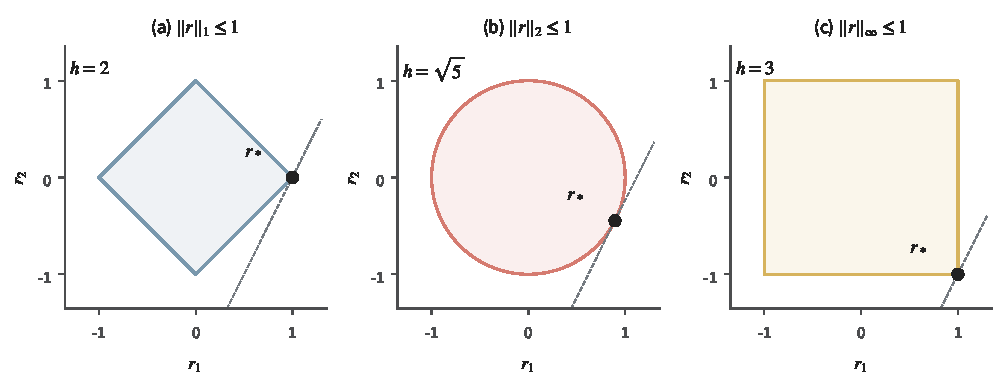
\includegraphics[width=\linewidth]{figures/math-preparation/concept-revision-linear-geometry/linear-dual-unit-balls.pdf}
 \caption{同一线性量$2r_1-r_2$在三种单位球上的最大值。实线是可行边界，灰虚线是达到最大值时的支撑直线，实心点给出一个最大化扰动。依次得到$2$、$\sqrt5$和$3$；由于单位球关于原点对称，最大绝对值相同，反方向也能达到。三个面板使用相同坐标尺度，图为解析教学示例。}
 \label{fig:linear-algebra-dual-unit-balls}
\end{figure*}

这里的“对偶”是相对于一个范数单位球最大化线性函数，从而为向量$\bm{z}$定义另一个范数。第~\ref{sec:opt-duality}节的拉格朗日对偶则从约束优化问题构造对偶函数和最优值下界，研究对象是原问题与对偶问题之间的关系。两者都出现线性配对，但定义、输出和用途不同，不能把对偶范数直接当作某个优化问题的拉格朗日对偶。

近共线坐标也可用这一语言观察。式\eqref{eq:linear-algebra-coordinate-instability}中第二个坐标为$\delta/\varepsilon$，所以目标沿$\bm{q}$方向改变$\Delta\delta$时，该坐标改变$\Delta\delta/\varepsilon$。这是特定坐标映射对该方向扰动的放大；要对所有方向给出统一上界，需要下一章引入矩阵的诱导范数和条件数。

\subsection{加权内积与半正定伪距离}

范数给所有位置使用同一套长度规则，矩阵则可以为不同方向指定不同权重。若实矩阵$\bm{M}\in\mathbb{R}^{d\times d}$对称正定，则
\[
  \langle\bm{x},\bm{y}\rangle_{\bm{M}}
  =
  \bm{x}^{\top}\bm{M}\bm{y},
  \qquad
  \lVert\bm{x}\rVert_{\bm{M}}
  =
  \sqrt{\bm{x}^{\top}\bm{M}\bm{x}}
\]
分别定义内积及其诱导范数。对称性给出内积的对称性，双线性来自矩阵乘法，正定性保证非零向量的平方长度严格为正；Cauchy--Schwarz不等式再保证三角不等式。因此
$d_{\bm{M}}(\bm{x},\bm{y})=\lVert\bm{x}-\bm{y}\rVert_{\bm{M}}$确实是距离。

欧氏距离对所有方向一视同仁，但有些问题需要让不同方向承担不同权重。设$\bm{M}\in\mathbb{R}^{d\times d}$为对称半正定矩阵，即对每个$\bm{z}\in\mathbb{R}^d$都有$\bm{z}^{\top}\bm{M}\bm{z}\geq0$。定义
\begin{equation}
  d_{\bm{M}}(\bm{x},\bm{y}) = \sqrt{ (\bm{x}-\bm{y})^{\top} \bm{M} (\bm{x}-\bm{y}) }. \label{eq:linear-algebra-mahalanobis-pseudodistance}
\end{equation}
若$\bm{M}=\bm{L}^{\top}\bm{L}$，那么$d_{\bm{M}}(\bm{x},\bm{y}) =\lVert\bm{L}(\bm{x}-\bm{y})\rVert_2$。因此非负性、对称性和三角不等式都继承自欧氏范数。

每个实对称半正定矩阵都存在这样的分解；第~\ref{sec:matrix-analysis-functions-structured-operations}节将构造方阵谱平方根$\bm{L}=\bm{M}^{1/2}\in\mathbb{R}^{d\times d}$。当$\bm{M}$正定时，这个方阵因子可逆，换坐标$\bm{x}\mapsto\bm{L}\bm{x}$把$\bm{M}$诱导的几何转成欧氏几何；半正定情形中$\bm{L}$可以消去非零方向，因而还要检查距离的可分辨性。

半正定性却不保证不同向量之间的距离为正。取
\[
  \bm{M}
  =
  \begin{bmatrix} 1&0\\0&0 \end{bmatrix}.
\]
点$(0,0)^{\top}$与$(0,1)^{\top}$不同，但它们的$d_{\bm{M}}$距离为$0$，因为第二个方向被完全忽略。为了描述这种丢失分辨力的几何，需要放宽距离的可分辨性条件。

这种允许不同点距离为零的比较方式，是定义~\ref{def:analysis-pseudometric}中的伪距离。半正定二次型保留距离的其余规则，丢失的只是对不同对象的分辨力。

只有当$\bm{M}$正定，也就是对所有非零$\bm{z}$均有$\bm{z}^{\top}\bm{M}\bm{z}>0$时，式\eqref{eq:linear-algebra-mahalanobis-pseudodistance}才区分任意两个不同向量，成为真正的距离。

权重矩阵改变的是几何判断。若用$\bm{M}$比较特征或表示，就应说明哪些方向被强调、哪些方向被忽略，以及这种选择为何适合当前任务。半正定矩阵造成的零距离不表示两个原始对象相等，只表示所选几何无法区分它们。

内积还规定“伴随”与“转置”的关系。定义~\ref{def:functional-adjoint}已在实Hilbert空间中建立伴随；有限维实内积空间自动完备，因而是它的特殊情形。这里也采用复内积空间中的同一配对定义，实空间时共轭转置退化为转置。伴随把输出上的线性配对搬回输入，由内积确定，不能仅靠交换矩阵行列来定义。

对$T:V\to W$，伴随$T^*:W\to V$满足
\[
 \langle T\bm x,\bm y\rangle_W=\langle\bm x,T^*\bm y\rangle_V
 \qquad(\bm x\in V,\ \bm y\in W)
\]
这一配对等式。

标准正交坐标中的伴随矩阵是共轭转置$\bm A^*$。若输入、输出坐标的内积分别由正定矩阵$\bm M_V$、$\bm M_W$给出，同一等式要求伴随矩阵为$\bm M_V^{-1}\bm A^*\bm M_W$。例如实矩阵$\bm A=\left[\begin{smallmatrix}0&1\\0&0\end{smallmatrix}\right]$在两端都采用$\bm M=\operatorname{diag}(1,4)$时，伴随矩阵为$\left[\begin{smallmatrix}0&0\\1/4&0\end{smallmatrix}\right]$，而普通转置的对应条目为$1$。因此第~\ref{sec:linear-algebra-matrices-linear-maps}节的共轭转置公式使用的是标准内积；更换几何后，伴随也须相应改变。

\section{正交投影与最小二乘}
\label{sec:linear-algebra-projection-least-squares}

\subsection{正交投影与最近点}

当线性方程$\bm{A}\bm{x}=\bm{b}$无解时，$\bm{b}$不在$\operatorname{col}(\bm{A})$中。若采用欧氏距离，一个自然替代问题是在列空间中寻找离$\bm{b}$最近的向量。设$U$是有限维内积空间$V$的线性子空间。\term{正交投影}（orthogonal projection）把$\bm{y}\in V$分解为
\[
  \bm{y}
  =
  \widehat{\bm{y}}+\bm{r},
  \qquad
  \widehat{\bm{y}}\in U,
  \quad
  \bm{r}\perp U.
\]
其中$\widehat{\bm{y}}$称为$\bm{y}$在$U$上的投影，$\bm{r}$是残差
\scite{math-axler2015linear}

有限维子空间自动是闭集。把定理~\ref{thm:functional-hilbert-projection}中的闭凸集
取为线性子空间$U$，便得到投影的存在唯一性；该章还证明了线性子空间情形的最近点
条件等价于残差正交，这里不再重复证明。正交性还直接给出最近点的距离分解：对任意
$\bm{u}\in U$，由于$\widehat{\bm{y}}-\bm{u}\in U$，
\[
  \lVert\bm{y}-\bm{u}\rVert^2
  =
  \lVert\bm{r}\rVert^2
  +
  \lVert\widehat{\bm{y}}-\bm{u}\rVert^2.
\]
第二项非负，且仅在$\bm{u}=\widehat{\bm{y}}$时为零，所以投影确实是$U$中的唯一最近点。有限维坐标仍可直接写出：取$U$的一组
标准正交基$(\bm{q}_1,\ldots,\bm{q}_r)$，则
\[
  \widehat{\bm{y}}
  =
  \sum_{j=1}^{r}
  \langle\bm{q}_j,\bm{y}\rangle\bm{q}_j.
\]
每个系数都是$\bm{y}$沿对应基方向的分量。

若$\bm{Q}\in\mathbb{F}^{m\times r}$的列组成$U$的一组标准正交基，即$\bm{Q}^{*}\bm{Q}=\bm{I}_r$，那么投影写成
\begin{equation}
  \widehat{\bm{y}} = \bm{Q}\bm{Q}^{*}\bm{y}, \qquad \bm{P}_U=\bm{Q}\bm{Q}^{*}. \label{eq:linear-algebra-orthogonal-projector}
\end{equation}
投影矩阵满足$\bm{P}_U^{*}=\bm{P}_U$和$\bm{P}_U^2=\bm{P}_U$：它是自伴的，而且投影一次后再次投影不会改变结果。

\subsection{残差正交与正规方程}

给定$\bm{X}\in\mathbb{R}^{n\times d}$和$\bm{y}\in\mathbb{R}^n$，\term{最小二乘}（least squares）问题是
\begin{equation}
  \min_{\bm{w}\in\mathbb{R}^d} \lVert\bm{X}\bm{w}-\bm{y}\rVert_2^2. \label{eq:linear-algebra-least-squares}
\end{equation}
所有拟合向量$\bm{X}\bm{w}$恰好组成$\operatorname{col}(\bm{X})$，所以
定理~\ref{thm:functional-hilbert-projection}保证最近的拟合向量总是存在且唯一。
即使系数$\bm{w}$不唯一，拟合向量也不会因此变成多个不同的最近点。

记最优拟合向量为$\widehat{\bm{y}}=\bm{X}\widehat{\bm{w}}$，残差为$\bm{r}=\bm{y}-\bm{X}\widehat{\bm{w}}$。残差与列空间正交，当且仅当它与$\bm{X}$的每一列正交，因此
\begin{equation}
  \bm{X}^{\top} (\bm{y}-\bm{X}\widehat{\bm{w}}) = \bm{0}, \qquad\text{即}\qquad \bm{X}^{\top}\bm{X}\widehat{\bm{w}} = \bm{X}^{\top}\bm{y}. \label{eq:linear-algebra-normal-equations}
\end{equation}
这就是\term{正规方程}（normal equations）。“正规”在这里指法向或正交关系，不表示矩阵已经归一化。

正规方程的系数矩阵$\bm X^{\top}\bm X$并非任意构造：它记录设计矩阵各列之间的内积。
把这一对象单独定义，便可以把“列是否冗余”转成一个方阵的正定性判断。
\begin{definition}[有限向量族的Gram矩阵]
\label{def:linear-algebra-gram-matrix}
设$\bm v_1,\ldots,\bm v_d$属于同一实或复内积空间。它们的\term{Gram矩阵}
（Gram matrix）为$\bm G\in\mathbb F^{d\times d}$，其中
$g_{i,j}=\langle\bm v_i,\bm v_j\rangle$。在标准坐标下，若这些向量是矩阵$\bm X$的列，
则$\bm G=\bm X^*\bm X$。
\end{definition}
对任意$\bm a\in\mathbb F^d$，有
$\bm a^*\bm G\bm a=\lVert\sum_j a_j\bm v_j\rVert^2\geq0$，
故Gram矩阵总是半正定；它正定当且仅当这些向量线性无关。这里比较的是列之间的关系，
不是每一列本身是否很大。

也可以直接从目标函数验证这一条件。对任意增量$\bm{h}$，
\begin{align*}
  \lVert\bm{X}(\widehat{\bm{w}}+\bm{h})-\bm{y}\rVert_2^2
  &=
  \lVert-\bm{r}+\bm{X}\bm{h}\rVert_2^2\\
  &=
  \lVert\bm{r}\rVert_2^2
  -2\bm{h}^{\top}\bm{X}^{\top}\bm{r}
  +\lVert\bm{X}\bm{h}\rVert_2^2.
\end{align*}
当式~\eqref{eq:linear-algebra-normal-equations}成立时，中间项为零，目标只能增加$\lVert\bm{X}\bm{h}\rVert_2^2$，所以正规方程不仅是驻点条件，也足以保证全局最优。

若$\operatorname{rank}(\bm{X})=d$，则对每个非零$\bm{z}$都有
\[
  \bm{z}^{\top}\bm{X}^{\top}\bm{X}\bm{z}
  =
  \lVert\bm{X}\bm{z}\rVert_2^2
  >0.
\]
于是$\bm{X}^{\top}\bm{X}$正定且可逆，系数解唯一：
\begin{equation}
  \widehat{\bm{w}} = (\bm{X}^{\top}\bm{X})^{-1}\bm{X}^{\top}\bm{y}. \label{eq:linear-algebra-full-rank-least-squares}
\end{equation}
若秩不足，存在非零$\bm{z}\in\operatorname{null}(\bm{X})$。任一最优系数$\widehat{\bm{w}}$与$\widehat{\bm{w}}+\bm{z}$给出相同拟合向量，所以系数不唯一。下一章将构造伪逆，并证明它在这些解中选择欧氏范数最小者。

\term{加权最小二乘}（weighted least squares）沿用同一个投影问题，但改用正定权重矩阵$\bm{M}\in\mathbb{R}^{n\times n}$衡量残差：
\[
  \min_{\bm{w}\in\mathbb{R}^d}
  (\bm{X}\bm{w}-\bm{y})^{\top}
  \bm{M}
  (\bm{X}\bm{w}-\bm{y}).
\]
此时“残差正交”指$\bm{M}$内积下的正交，即
\begin{equation}
  \bm{X}^{\top}\bm{M}
  (\bm{y}-\bm{X}\widehat{\bm{w}})
  =
  \bm{0},
  \qquad
  \bm{X}^{\top}\bm{M}\bm{X}\widehat{\bm{w}}
  =
  \bm{X}^{\top}\bm{M}\bm{y}.
  \label{eq:linear-algebra-weighted-normal-equations}
\end{equation}
正定性使这仍是列空间上的正交投影，最优拟合向量存在且唯一；系数仍在$\bm{X}$满列秩时才唯一。若权重矩阵仅半正定，目标可能完全忽略某些残差方向，前述唯一性结论便不能直接沿用。

\begin{example}[同一子空间的两种最近点]
\label{ex:linear-algebra-weighted-projection}
令$\bm b=(2,1)^{\top}$，子空间由$\bm v=(1,1)^{\top}$张成。欧氏投影为
$\bm p=\bm v(\bm v^{\top}\bm b)/(\bm v^{\top}\bm v)=(1.5,1.5)^{\top}$。
若改用$\bm M=\operatorname{diag}(1,4)$，投影系数为
$(\bm v^{\top}\bm M\bm b)/(\bm v^{\top}\bm M\bm v)=6/5$，
故$\bm p_{\bm M}=(1.2,1.2)^{\top}$。第二坐标误差更昂贵，因此最近点向$b_2=1$靠近。
残差$\bm b-\bm p_{\bm M}=(0.8,-0.2)^{\top}$与$\bm v$的普通内积不是零，
但$\bm v^{\top}\bm M(\bm b-\bm p_{\bm M})=0$，仍满足所选内积下的正交性。
\end{example}

\begin{figure*}[htbp]
 \centering
 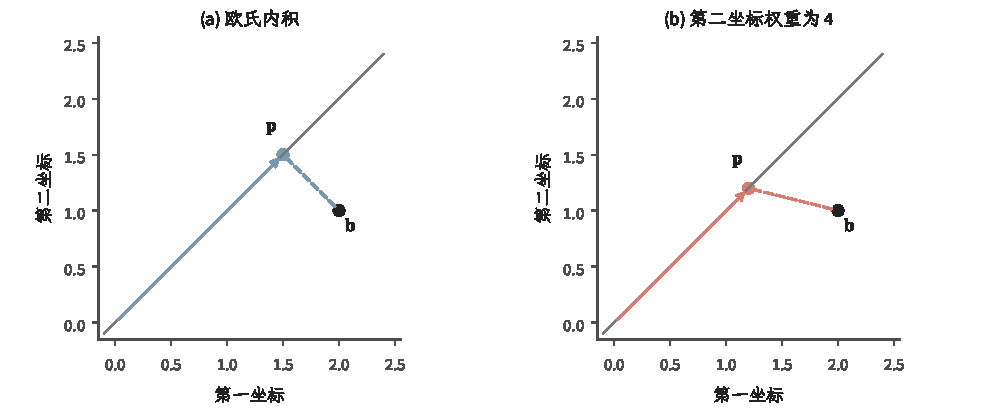
\includegraphics[width=\linewidth]{figures/math-preparation/analysis-geometry/linear-algebra-weighted-projection.pdf}
 \caption{例~\ref{ex:linear-algebra-weighted-projection}的两个最近点。灰直线是同一个子空间，黑点是同一目标向量，实箭头指向投影，虚线连接残差。右图中的欧氏角度不必为直角，正交性由加权内积判断。两图坐标比例相同。}
 \label{fig:linear-algebra-weighted-projection}
\end{figure*}

\subsection{近共线问题中的系数、拟合与残差}

回到$\bm{X}_{\varepsilon}$与$\bm{y}$。由于$\bm{c}_1^{\top}\bm{q}=0$且$\lVert\bm{q}\rVert_2^2=2$，
\[
  \bm{X}_{\varepsilon}^{\top}\bm{X}_{\varepsilon}
  =
  \begin{bmatrix} 3&3\\ 3&3+2\varepsilon^2 \end{bmatrix},
  \qquad
  \bm{X}_{\varepsilon}^{\top}\bm{y}
  =
  \begin{bmatrix} 3\\ 3+2\varepsilon\delta \end{bmatrix}.
\]
这里的Gram矩阵由定义~\ref{def:linear-algebra-gram-matrix}得到，其行列式为$6\varepsilon^2$。当$\varepsilon\neq0$时，正规方程唯一解为
\begin{equation}
  \widehat{\bm{w}}_{\varepsilon} = \begin{bmatrix} 1-\delta/\varepsilon\\ \delta/\varepsilon \end{bmatrix}, \qquad \bm{X}_{\varepsilon}\widehat{\bm{w}}_{\varepsilon} = \bm{y}. \label{eq:linear-algebra-nearly-collinear-least-squares}
\end{equation}
这与式~\eqref{eq:linear-algebra-coordinate-instability}一致。取$\varepsilon=0.01$和$\delta=0.1$，系数为$(-9,10)^{\top}$，拟合残差却恰为零。因此“大系数”和“大训练残差”是不同判断。

再令$\varepsilon=0$。此时列空间退化为$U=\operatorname{span}\{\bm{c}_1\}$，而$\bm{y}=\bm{c}_1+\delta\bm{q}$已经是正交分解。投影与残差分别为
\[
  \widehat{\bm{y}}_0=\bm{c}_1,
  \qquad
  \bm{r}_0=\delta\bm{q},
  \qquad
  \lVert\bm{r}_0\rVert_2^2=2\delta^2.
\]
所有满足$w_1+w_2=1$的系数都给出同一个拟合向量$\bm{c}_1$。系数解有无穷多个，但最优拟合向量仍唯一；同时，$\delta\bm{q}$方向已经不在列空间中，所以不可能把残差降为零。

这个边界还说明一个不连续现象：对每个非零$\varepsilon$，矩阵都能精确拟合$\bm{y}$，但所需系数的范数随着$\varepsilon\to0$而发散；在极限矩阵$\bm{X}_0$上，目标又不再能够精确拟合。矩阵元素接近并不保证方程解接近。下一章将用小奇异值与条件数定量解释这种敏感性，并比较正则化和稳定求解保留了什么。

\section{多维数组与结构运算}
\label{sec:linear-algebra-tensors-structured-operations}

最小二乘已经展示了两个索引上的线性组合。图像、多个样本和多组通道只是增加了索引轴，
每一次运算仍需说明哪些轴被汇总、哪些轴留下。这里把数组作为坐标数据组织起来，
不预设读者已学过抽象张量代数；注意力和卷积的例子用于核对索引，而非提前建立模型。

\subsection{组织索引轴与消去共同索引}

\subsubsection{多维数组的形状与索引}

向量有一个坐标索引，矩阵有行列两个索引。机器学习中的一批序列、图像或特征图还需要批次、位置、通道等更多索引。要正确运算，必须先明确每个元素由哪些索引定位。
\begin{definition}[多维数值数组]
\label{def:linear-algebra-multidimensional-array}
给定正整数$n_1,\ldots,n_k$，一个形状为$n_1\times\cdots\times n_k$的数值数组，
是从有限索引集$\{1,\ldots,n_1\}\times\cdots\times\{1,\ldots,n_k\}$到
$\mathbb F$的映射。第$j$个索引称为第$j$个轴，轴数$k$称为数组的阶。
本节沿用机器学习中的常见说法，将这种多维数组称为\term{张量}（tensor）。
\end{definition}
例如
\[
  \bm{X}\in
  \mathbb{R}^{b\times \ell\times d}
\]
表示含$b$个样本、每个样本有$\ell$个位置、每个位置有$d$个特征的数组，$x_{i,j,k}$是第$i$个样本、第$j$个位置的第$k$个特征。这里的“阶”指索引轴数量，不应与矩阵秩或高阶张量分解中的各种秩混淆。

这种用法描述的是数组的存储形状。几何中的张量对象还必须规定换基时各个坐标索引怎样共同变换，使不同基下的分量表示同一个多线性对象；只有形状相同并不能保证数组满足这种变换规律。本节只需要数组及其索引运算，后文若使用坐标无关的张量对象，将另行说明相应的空间与换基规则。

形状不仅是存储信息，也说明某个运算对哪些索引求和、保留哪些索引。若$\bm{X}\in\mathbb{R}^{b\times\ell\times d}$且$\bm{W}\in\mathbb{R}^{d\times h}$，对最后一维应用同一个线性映射得到
\[
  z_{i,j,r}
  =
  \sum_{k=1}^{d}x_{i,j,k}w_{k,r},
  \qquad
  \bm{Z}\in\mathbb{R}^{b\times\ell\times h}.
\]
索引$k$被求和并消失，批次索引$i$、位置索引$j$和输出特征索引$r$保留下来。

\term{维度重排}（permutation of axes）只改变索引次序，例如把$b\times\ell\times d$改为$b\times d\times\ell$；\term{形状重整}（reshape）则在元素总数不变时重新组织索引。它们可以不改变底层数值，却会改变后续运算如何解释各轴。把通道轴误当作位置轴，即使元素数量仍匹配，也会计算另一个映射。因此每次重排都应同时保留各轴的语义，而不能只核对总元素数。

\subsubsection{缩并与逐元素乘法}

\term{张量缩并}（tensor contraction）选取两个或多个索引轴，逐项相乘并对这些轴求和。矩阵乘法\eqref{eq:linear-algebra-matrix-product}就是沿一个共同索引的缩并。更一般地，若
\[
  \bm{A}\in\mathbb{R}^{m\times d\times r},
  \qquad
  \bm{B}\in\mathbb{R}^{d\times n\times r},
\]
沿第二个数组的第一轴与共同的$r$轴缩并可定义
\[
  c_{i,j}
  =
  \sum_{k=1}^{d}\sum_{s=1}^{r}
  a_{i,k,s}b_{k,j,s},
  \qquad
  \bm{C}\in\mathbb{R}^{m\times n}.
\]
写出索引能直接说明哪些维度必须相等，也能避免把本应保留的轴错误求和。

两个同形数组的\term{逐元素乘积}（Hadamard product）记作$\bm{A}\odot\bm{B}$，定义为
\[
  (\bm{A}\odot\bm{B})_{i,j}=a_{i,j}b_{i,j}.
\]
它保留原形状，不对索引求和，所以通常不同于矩阵乘法。例如
\[
  \begin{bmatrix} 1&2\\3&4 \end{bmatrix}
  \odot
  \begin{bmatrix} 0&1\\1&0 \end{bmatrix}
  =
  \begin{bmatrix} 0&2\\3&0 \end{bmatrix},
\]
而同样两矩阵的矩阵乘积为$\left[\begin{smallmatrix}2&1\\4&3\end{smallmatrix}\right]$。门控常使用逐元素乘法，线性层则使用缩并；二者不能因为都写了“乘”而互换。

\begin{table*}[htbp]
 \centering\small
 \begin{tabularx}{\linewidth}{@{}lXX@{}}
 \toprule
 运算 & 形状条件与输出 & 索引上的含义\\
 \midrule
 $\bm A\bm B$ & $(m\times n)(n\times p)\to m\times p$ & 对共同索引求和：$c_{i,k}=\sum_j a_{i,j}b_{j,k}$\\
 $\bm A\odot\bm B$ & 两者均为$m\times n$，输出$m\times n$ & 相同索引逐元素相乘，不求和\\
 $\bm A\otimes\bm B$ & $(m\times n)$与$(p\times q)\to(mp)\times(nq)$ & 保留两组成对索引，生成分块矩阵\\
 $\bm x^{\top}\bm y$ & 两个实$n$维向量，输出标量 & 对唯一共同索引求和\\
 \bottomrule
 \end{tabularx}
 \caption{相乘符号的不同含义。形状检查先确定哪些索引被消去，再确定结果对应什么对象。}
 \label{tab:linear-algebra-products-and-shapes}
\end{table*}

\subsection{方阵缩并与乘积结构}

矩阵有两个索引，仍可从数组角度观察它。迹把两个索引对齐后求和，Kronecker积则保留两组
索引并组成分块矩阵。二者分别解决“汇总同一映射的对角作用”和“组合两个独立轴上的作用”，
不是矩阵乘法的同义写法。

\subsubsection{矩阵迹}

方阵$\bm{A}\in\mathbb{F}^{d\times d}$的\term{迹}（trace）定义为
\[
  \operatorname{tr}(\bm{A})
  =
  \sum_{j=1}^{d}a_{j,j}.
\]
迹是对两个矩阵索引施加相等约束后求和的缩并。只要乘积维度相容，
\begin{equation}
  \operatorname{tr}(\bm{A}\bm{B}) = \operatorname{tr}(\bm{B}\bm{A}), \label{eq:linear-algebra-trace-cyclic}
\end{equation}
因为
\[
  \operatorname{tr}(\bm{A}\bm{B})
  =
  \sum_i\sum_j a_{i,j}b_{j,i}
  =
  \sum_j\sum_i b_{j,i}a_{i,j}.
\]
对三个以上因子，可以循环移动因子，但不能任意交换次序：$\operatorname{tr}(\bm{A}\bm{B}\bm{C}) =\operatorname{tr}(\bm{B}\bm{C}\bm{A})$，一般却不等于$\operatorname{tr}(\bm{A}\bm{C}\bm{B})$。

迹还把矩阵空间上的标准内积写成
\[
  \langle\bm{A},\bm{B}\rangle_{\mathrm{F}}
  =
  \operatorname{tr}(\bm{A}^{*}\bm{B})
  =
  \sum_{i,j}\overline{a_{i,j}}b_{i,j}.
\]
由此诱导的Frobenius范数为$\lVert\bm{A}\rVert_{\mathrm{F}} =\sqrt{\sum_{i,j}|a_{i,j}|^2}$。它把矩阵全部元素排成一个向量后计算欧氏长度；下一章会把它与控制最大方向伸缩的算子范数区分开。

\subsubsection{Kronecker积}

设$\bm{A}\in\mathbb{F}^{m\times n}$，$\bm{B}\in\mathbb{F}^{p\times q}$。它们的\term{Kronecker积}（Kronecker product）是分块矩阵
\begin{equation}
  \bm{A}\otimes\bm{B} = \begin{bmatrix} a_{1,1}\bm{B}&\cdots&a_{1,n}\bm{B}\\ \vdots&\ddots&\vdots\\ a_{m,1}\bm{B}&\cdots&a_{m,n}\bm{B} \end{bmatrix} \in\mathbb{F}^{mp\times nq}. \label{eq:linear-algebra-kronecker-product}
\end{equation}
它不是逐元素乘积，也不是普通矩阵乘法，而是把两个索引系统组合成一个较大的线性映射。
例如，$\bm{A}$可以描述第一个索引上的作用，$\bm{B}$描述第二个索引上的作用，
$\bm{A}\otimes\bm{B}$则把两种作用组合到成对索引上。第
~\ref{sec:matrix-analysis-blocks-updates}节将统一定义矩阵向量化，
完整推导它与Kronecker积的恒等式，并说明何时可以利用乘积结构而不显式构造大矩阵。

\subsection{加权读取与局部读取的索引核对}

基本缩并规则可用于不同的信息读取方式：一次输出可以对全部候选位置加权，也可以只读取一个
固定大小的邻域。以下两例只检验索引、权重与输出之间的关系；模型怎样从数据得到这些权重，
留在后续模型章讨论。

\subsubsection{注意力中的索引缩并}

一个小型\term{注意力}（attention）计算可以显示形状如何决定运算。设有$\ell$个位置，查询与键的维数为$d_k$，值的维数为$d_v$：
每个查询向量描述当前位置要匹配的特征，键向量用于给候选位置打分，值向量才是被加权读取的内容。
因此查询与键需要共享特征维数，值的维数可以不同。
\[
  \bm{Q},\bm{K}\in\mathbb{R}^{\ell\times d_k},
  \qquad
  \bm{V}\in\mathbb{R}^{\ell\times d_v}.
\]
分数矩阵与逐行归一化权重定义为
\begin{align}
  \bm{S}
  &=
  \frac{\bm{Q}\bm{K}^{\top}}{\sqrt{d_k}}
  \in\mathbb{R}^{\ell\times\ell},
  \label{eq:linear-algebra-attention-scores}\\
  a_{i,j}
  &=
  \frac{\exp(s_{i,j})}
       {\sum_{r=1}^{\ell}\exp(s_{i,r})},
  \qquad
  \bm{O}
  =
  \bm{A}\bm{V}
  \in\mathbb{R}^{\ell\times d_v}.
  \label{eq:linear-algebra-attention-contraction}
\end{align}
式~\eqref{eq:linear-algebra-attention-scores}沿特征索引缩并，留下两个位置索引；式\eqref{eq:linear-algebra-attention-contraction}再沿被读取的位置索引缩并，留下查询位置与值特征索引。权重每行和为$1$，在这里表示归一化加权平均；概率语义需要另有随机对象支持，不能只由非负且和为$1$推出。

查询数和键数也可以不同。取两个二维查询、三条二维键和三个标量值，
\[
  \bm{Q}
  =
  \begin{bmatrix}
    1&0\\
    0&1
  \end{bmatrix}
  \in\mathbb{R}^{2\times2},
  \qquad
  \bm{K}
  =
  \begin{bmatrix}
    1&0\\
    0&1\\
    1&1
  \end{bmatrix}
  \in\mathbb{R}^{3\times2},
  \qquad
  \bm{V}
  =
  \begin{bmatrix}v_1\\v_2\\v_3\end{bmatrix}
  \in\mathbb{R}^{3\times1}.
\]
共同的特征维数$2$被缩并，故
\[
  \bm{Q}\bm{K}^{\top}
  =
  \begin{bmatrix}
    1&0&1\\
    0&1&1
  \end{bmatrix}
  \in\mathbb{R}^{2\times3}.
\]
逐行归一化得到$\bm{A}\in\mathbb{R}^{2\times3}$后，输出$\bm{A}\bm{V}\in\mathbb{R}^{2\times1}$；其中每一行都是$v_1,v_2,v_3$的一次加权缩并。这个例子把“共同特征轴”和“三条被读取的位置轴”分开，说明可乘条件来自被缩并轴，而不要求查询数等于键数。

取$\ell=d_k=d_v=2$，
\[
  \bm{Q}=\bm{K}=\bm{I}_2,
  \qquad
  \bm{V}
  =
  \begin{bmatrix} 1&1\\ 1&1+\varepsilon \end{bmatrix}.
\]
记$c=\exp(1/\sqrt{2})$，则
\[
  \bm{A}
  =
  \frac{1}{c+1}
  \begin{bmatrix} c&1\\ 1&c \end{bmatrix},
  \qquad
  \bm{O}
  =
  \begin{bmatrix} 1&1+\varepsilon/(c+1)\\ 1&1+c\varepsilon/(c+1) \end{bmatrix}.
\]
按列比较可得
\[
  \bm{O}_{:,2}-\bm{O}_{:,1}
  =
  \frac{\varepsilon}{c+1}
  \begin{bmatrix}1\\c\end{bmatrix},
\]
所以值矩阵的两列接近时，输出两列之差仍为$O(|\varepsilon|)$。按行看，$\bm{V}$的每一行才是一个位置上的值向量，并且
$\bm{O}_{i,:}=\sum_j a_{i,j}\bm{V}_{j,:}$。因此每个输出行都是原值向量的加权平均，属于$\operatorname{row}(\bm{V})$；这个行空间结论与前面的列差关系讨论的是两个不同的索引方向。

\subsubsection{卷积中的局部缩并}

\term{卷积}（convolution）也可写成索引缩并，但它只连接局部位置，并在不同位置复用同一组核参数。设一个二维输入窗口为$\bm{U}\in\mathbb{R}^{k_h\times k_w\times c_{\mathrm{in}}}$，卷积核为
\[
  \bm{K}\in
  \mathbb{R}^{k_h\times k_w\times c_{\mathrm{in}}\times c_{\mathrm{out}}}.
\]
忽略偏置时，该窗口产生的第$r$个输出通道为
\begin{equation}
  z_r = \sum_{a=1}^{k_h} \sum_{b=1}^{k_w} \sum_{s=1}^{c_{\mathrm{in}}} u_{a,b,s}k_{a,b,s,r}. \label{eq:linear-algebra-convolution-window-contraction}
\end{equation}
三个输入索引被缩并，输出通道索引$r$保留。把窗口移动到另一个位置时，输入元素改变，核参数不变；边界如何补齐、步幅多大以及这里采用卷积还是相关的索引方向，都需要在具体模型中另行说明。

取一个长度为$2$、含两个通道的一维窗口
\[
  \bm{U}
  =
  \begin{bmatrix} 1&1\\ 1&1+\varepsilon \end{bmatrix}.
\]
若核$\bm{K}_1$的两个位置都取第一通道并赋权$1/2$，输出为$1$；若核
\[
  \bm{K}_2
  =
  \begin{bmatrix} 0&-1\\ 0&1 \end{bmatrix},
\]
则缩并结果为$\varepsilon$，它提取第二通道在两个位置间的局部变化。前者保留共同方向，后者检测两行之间很小的差异。共享局部核规定了要从每个窗口读取的关系，但这些关系是否适合任务，还取决于输入轴的语义与边界设定。

高阶数组仍可视为一个向量空间中的对象，重排、逐元素乘法和缩并则是不同的运算。某些张量分解会进一步讨论能否用少量因子表示高阶数组，但高阶张量的“秩”存在多种不等价定义，也不像矩阵秩那样共享一套简单结论。本章只建立后续注意力、卷积和结构矩阵所需的形状与运算语言；具体分解在确有需要时再给出相应定义和条件。

\section{本章小结}
\label{sec:linear-algebra-summary}

线性代数把表示问题拆成几个不能混同的层次。向量是空间中的对象，坐标是对象相对于一组基的系数；线性映射描述作用，矩阵是它在输入、输出基下的表示。张成空间回答哪些输出可以表示，零空间回答哪些输入差异会被消去，秩零度定理把两者联系起来。换基会改变坐标和矩阵元素，却不改变这些空间关系。

内积、范数和正定度量进一步规定怎样比较方向、长度与误差。对偶范数精确给出指定范数球中线性变化的最大值；半正定矩阵可能忽略某些方向，所以只能给出伪距离。正交投影则在选定内积后找到子空间中的唯一最近向量。由此得到的最小二乘拟合向量总是唯一，但系数只有在设计矩阵列满秩时唯一。

贯穿本章的近共线样本显示了这些区别为何必要。$\varepsilon\neq0$时，两列特征线性无关，能够精确表示目标；随着$\varepsilon$趋近$0$，表示同一目标所需的系数却不断增大；到$\varepsilon=0$时，系数不唯一，而且原来沿$\bm{q}$方向的目标分量无法拟合。多维数组中的缩并、迹、Kronecker积、注意力和卷积仍建立在同样的线性组合与索引规则上，形状相容只保证运算有定义，不保证它保留了任务需要的信息。

本章已经说明哪些方向可表示、哪些误差按给定几何衡量，却还没有定量回答线性映射沿不同方向放大或压缩多少。下一章将用特征值、奇异值、矩阵范数和条件数分析这一问题，并据此解释近共线系统中的低秩近似、伪逆、扰动与稳定求解。
